In order to establish communication between the Arduino and the gateway, we need to prepare both components.
To prepare the gateway to act as an interface between the Arduino and the cloud, I registered it with The Things Network and followed the \href{https://www.thethingsnetwork.org/docs/gateways/multitech/aep.html}{instructions} provided by The Things Network.

Once all of the components are registered with The Things Network, we can set up our Arduino.
After logging into The Things Network's website, we need to navigate to the ``Applications'' pane.
This will allow us to get the necessary information to allow our Arduinos to join the LoRa network.
We need a device EUI, an application EUI, and an application key in order for the Arduino to join the network.
These are available on the console, as shown in \cref{fig:console}\footnote{The app key has been blurred out, as it should be kept secure to prevent new devices from being added to the network without administrator permission.}.
\begin{figure}[ht]
  \centering
  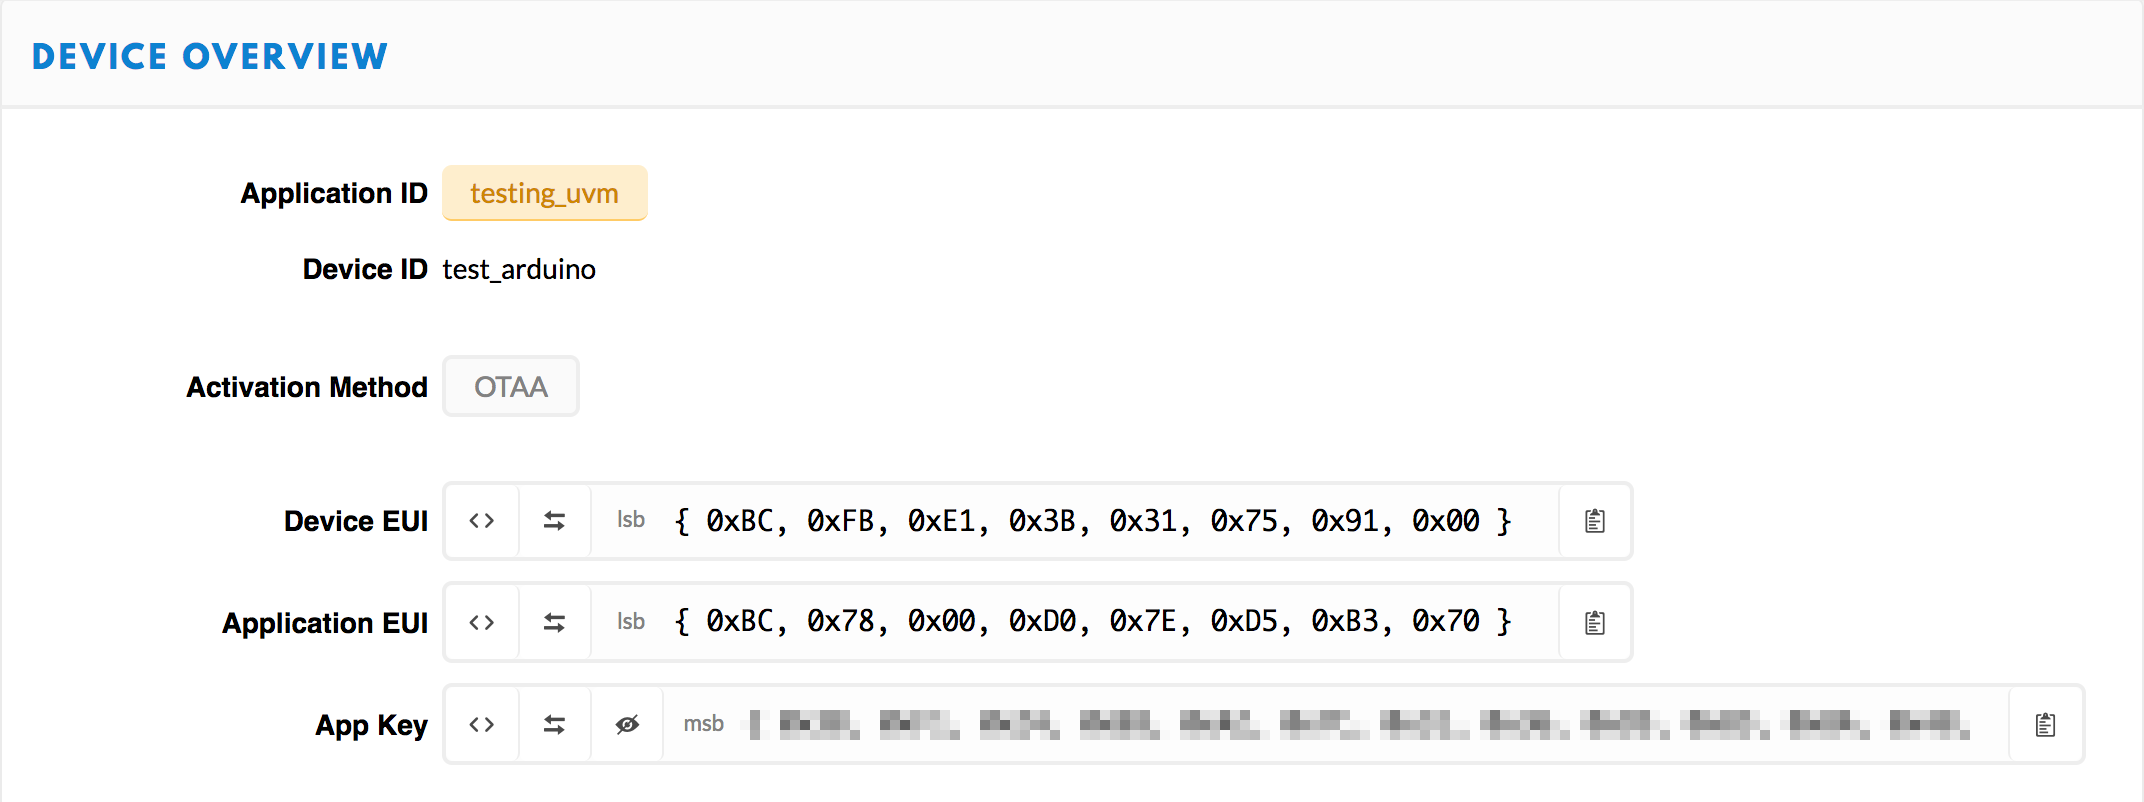
\includegraphics[width=\textwidth]{figure/console}
  \caption{The device overview from The Things Network console.}
  \label{fig:console}
\end{figure}

These get put into the over-the-air-activation (OTAA) script at \url{arduino/ttn_otaa/ttn_otaa.ino} as shown in \cref{fig:script}.
\begin{figure}[ht]
  \centering
  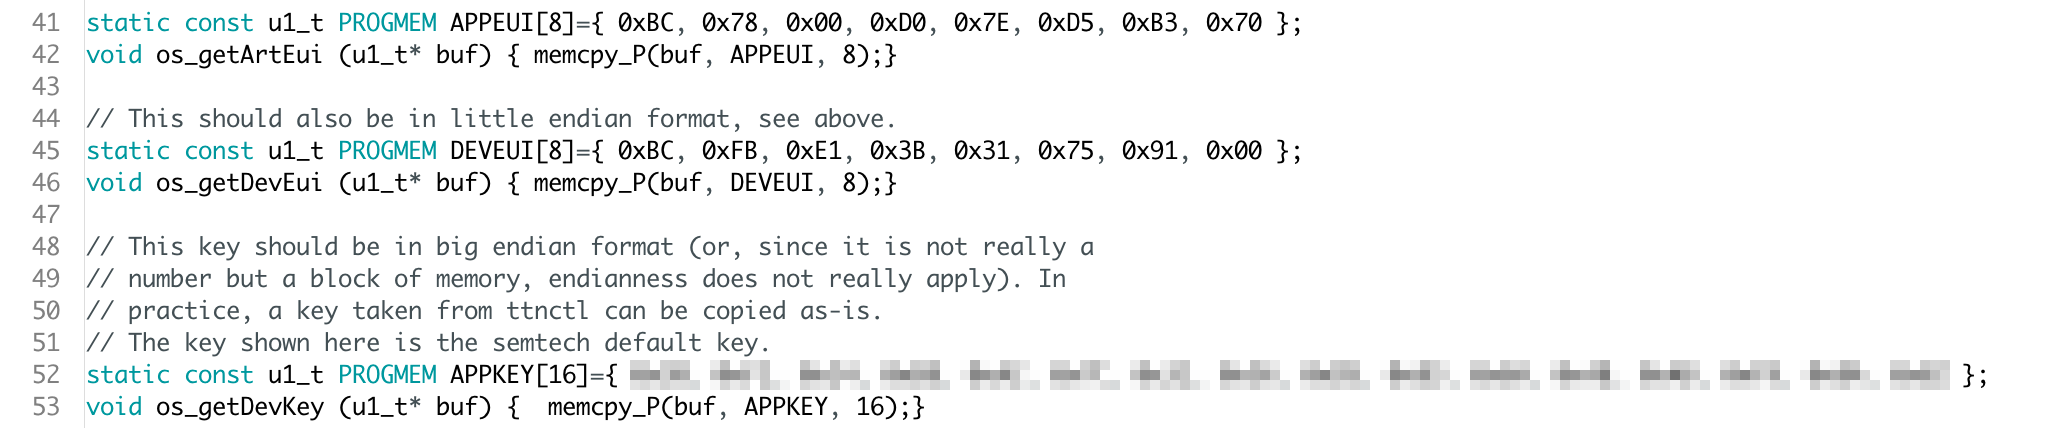
\includegraphics[width=\textwidth]{figure/script}
  \caption{The placement of the information from the The Things Network console.}
  \label{fig:script}
\end{figure}
Once these edits have been made, the script is uploaded to the Arduino, which tries to join the network established by the gateway.

%%% Local Variables:
%%% mode: latex
%%% TeX-master: "../writeup"
%%% End:
